\chapter{Architektúra ako celok}

Architektúra aplikácie má mriežkovú štruktúru. Je tvorená horizontálnymi (MVVM návrhový vzor) a~vertikálnymi (\textit{session}-y + hlavné okno) vrstvami. V~následujúcich sekciách popíšeme, ako jednotlivé vrstvy vyzerajú, aké sú ich úlohy a~ako medzi sebou komunikujú. Na~konci kapitoly je následne k~nahliadnutiu Diagram~\ref{obr02:priklad_struktury} znázorňujúci príklad možnej architektúry aplikácie.   

\section{MVVM(MV) návrhový vzor}\label{MVVMNavrhovyVzor}

Ako už bolo spomenuté v~Podsekcii~\ref{ArchitekturaMVVM}, v~aplikácii je využívaný návrhový vzor MVVM s~drobnou obmenou. Táto obmena sa týka rozdelenia originálnej vrstvy View model do~dvoch častí: View model a~Model view. Toto rozdelenie zaručí ešte o~niečo lepšiu separáciu kódu a~odľahčí tým úlohy View model vrstvy. 

MVVM(MV) architektúra teda rozdeluje aplikáciu na~4~vrstvy: View, ViewModel, ModelView a~Model. Popis jednotlivých vrstiev je k~nahliadnutiu v~následujúcich podsekciách. 

\subsection{View}

View je vrstva, ktorá popisuje a~implementuje grafickú stránku aplikácie a~určuje, akým spôsobom sa dáta dodané vrstvou View model zobrazia užívateľovi. View-y sú objekty viazané na~odpovedajúce view model-y za~pomoci reaktívneho programovania. Spracovávajú akcie užívateľa a~iniciujú reakcie zvyšných vrstiev architektúry prostredníctvom príslušného view model-u. Následne zabezpečujú zobrazovanie dodaných výsledkov reakcie.

View vrstva je implementovaná za~pomoci Avalonia UI framework-u. V~náväznosti na~tento fakt sú v~aplikácii použité tri hlavné typy view-ov:
\begin{itemize}
    \item \textbf{Window} - Reprezentujú špecifické okná aplikácie, \uv{top-level} kontajnery, ktoré~v~sebe držia nejaký obsah. Okná sami o~sebe nedefinujú vzhľad aplikácie. Slúžia predovšetkým ako rám, v~ktorom sa striedajú jednotlivé view-y. Každé okno má naviazaný svoj vlastný view model, ktorý~drží informáciu o~tom, aký view je v~danej chvíli v~okne zobrazovaný. Naviazaný view model taktiež obsahuje vlastnosti, ktoré~priamo súvisia s~vlastnosťami daného okna.
    \item \textbf{View} - Sú to hlavné zložky, ktoré~nesú grafiku zobrazujúcu sa oknách. Reprezentujú \uv{pohľady}, ktoré~sú užívateľovi vykresľované. Každý view je naviazaný na~špecifický view model. Viaže sa na~jeho vlastnosti a~reaktívne vykresluje dáta, ktoré~tieto vlastnosti nadobúdajú. 
    
    Býva zvykom že~sa konkrétny view zobrazuje práve v~jednom konkrétnom okne. V~takom prípade si na~jeho view model drží referenciu view model daného okna. Za~pomoci tejto referencie potom dokáže oknu jeho view model oznámiť, že~sa v~ňom má daný view zobraziť. 
    \item \textbf{DataTemplate} - Definuje grafickú reprezentáciu dát dodávaných z~View model vrstvy do~vrstvy View. Pre~každý dátový typ, ktorý~chce byť správne vykreslený pre~užívateľa, musí existovať špecifický dátový template, pomocou ktorého sa daný údaj vykreslí. Dátové template-y sú špecifické tým, že~sú raz definované pre~celú aplikáciu, aby~sa zachovala konzistencia vykreslovania jednotlivých dátových typov.

    Je potrebné podotknúť, že~na~to aby~údaj vygenerovaný vo~vrstve Model bolo možné vykresliť, musí preňho najprv existovať tzv. \textit{data view model} do~ktorého sú jeho informácie zabalené a~až v~takejto podobe predávané nejakému view model-u, ktorý~ich následne pomocou svojich vlastností odovzdá view-u na~vykreslenie. Pre~každý dátový view model sa následne hľadá príslušný DataTemplate, pomocu ktorého v~ňom držané informácie zobrazia užívateľovi. 
\end{itemize}   

View vrstva je implementovaná pomocou dvoch jazykov: C\# a~XAML. Pomocu XAML definujeme všetky polohy a~tvary grafických objektov a~bind-ujeme vlastnosti týchto objektov na~vlastnosti z~vrstvy View model. Pre~každý view máme obecne jeden špecifický XAML súbor ktorým ho implementujeme. K~väčšine XAML súborov je priradený C\# zdrojový súbor v~ktorom sa implementuje takzvaný \textit{code-behind}. V~tomto zdrojovom súbore môžeme doplniť všetku funkcionalitu view-u, ktorú nebolo možné vyjadriť jazykom XAML.    

\subsection{View model}\label{ViewModel}

Druhou v~poradí je vrstva View model. Táto vrstva je zodpovedná za~logiku spracovania akcií užívateľa oznámených reaktívnym spôsobom View vrstvou. Disponuje vedomím toho, aké akcie a~v~akom poradí sa majú vykonať pre~zabezpečenie správnej reakcie na~detegovaný impulz. K~tomuto účelu využíva služby nižších vrstiev prostredníctvom volania metód na~vrstve Model view. Tá na~základe svojej vnútornej logiky vráti odpoveď s~požadovanými údajmi. View model následne spracuje dodané dáta a~predostrie ich vrstve View, aby~ich mohla zobraziť užívateľovi.

View model na~základe aplikačnej logiky koriguje a~obmedzuje akcie užívateľa a~tým zabraňuje vzniku nekonzistentných stavov aplikácie. Taktiež v~niektorých prípadoch iniciuje \textit{interakcie} s~inými view model-mi za~účelom získania ich doplňujúcich služieb do~jeho vlastného procesu.


Podobne ako vo~View vrstve sa view model-y delia na~tri základné typy:
\begin{itemize}
    \item \textbf{Session view model (Main window view model)} - Odpovedajú jednotlivým \textit{session}-om, ktoré~sú základným kameňom vertikálnej štruktúry aplikácie. Viac informácií o~session-och je možné nájsť v~Sekcii~\ref{Sessions}. Výnimkou je práve \textit{Main window view model}, ktorý~je naviazaný na~hlavné okno aplikácie a~zabezpečuje preň aplikačnú logiku. Klasické session view model-y sú taktiež naviazané zvyčajne na~jedno okno z~vrstvy View, pre~ktoré zabezpečujú aplikačnú logiku.
    
    Každý session view model obsahuje kolekciu príslušných view model-ov, ktoré~spoločne implementujú mechanizmus daného session-u. Je zvykom, že~v~jednej chvíli je aktívny iba jeden view model. O~aktívnom view model-e je informované okno viazané na~daný session view model. To následne v~sebe zobrazuje odpovedajúci view aktívneho view model-u. Informovanie o~aktívnom view model-e je hlavnou pracovnou náplňou session view model-u.

    K~ďalším jeho povinnostiam patrí spracovávanie užívateľom vyvolaných akcií, ktoré~sa týkajú samotného naviazaného okna. Príkladom takej akcie môže byť požiadavka o~zatvorenie dotyčného okna.
    \item \textbf{View model} - Reprezentujú zložky, ktorých funkcionalita sa najväčšmi ponáša na~obecnú, vyššie popísanú funkcionalitu vrstvy View model. Väčšina view model-ov spadá pod réžiu konkrétneho session-u (alebo hlavného okna), pre~ktorý implementuje určitú časť jeho mechanizmu. Klasicky sú view model-y naviazané na~príslušné view-y z~vrstvy View. s~tými následne reaktívne komunikujú a~reagujú na~ich podnety. View model-y sú navzájom nezávislé. To znamená, že~medzi nimi neprebieha takmer žiadna komunikácia ani presun dát. Túto funkciu na~seba berie Model view vrstva.

    Väčšina view model-ov by mala byť zahrnutá v~zodpovedajúcom session view model-e (poprípade Main window view model-e). Ten potom zabezpečuje správu toho, ktorý~view model je v~danej chvíli aktívny. 
    
    Výnimkou sú view model-y, ktoré~sú výhradne používane pre~interakcie z~iných view model-ov, ktorým týmto spôsobom doručujú svoje služby. Tieto view model-y sú väčšinou vytvorené na~mieste interakcie a~po jej skončení zanikajú. Pri~ich vytváraní im sú zvyčajne predané nejaké vstupné parametre a~keď je ich práca dokončená, vracajú jej výsledok. 
    \item \textbf{Data view model} - slúžia ako kontajnery pre~informácie abstrahované z~dát vygenerovaných v~Model vrstve. Dáta sú klasicky konvertované do~ich zodpovedajúcich view model-ov v~Model view vrstve a~už takto zabalené informácie sú predávané do~View model vrstvy, kde sú spracované a~pomocou vlastností odovzdané vrstve View na~zobrazenie. Data view model-y môžu dodané informácie drobne upravovať takým spôsobom, aby~ich bolo jednoduchšie zobrazovať vo~View vrstve.
    
    Z~toho vyplýva, že~na~to, aby~nejaký údaj vygenerovaný v~Model vrstve mohol byť prezentovaný užívateľovi, musí preňho existovať odpovedajúci data view model. Zároveň na~to, aby~informácie obsiahnuté v~dátovom view model-e mohli byť vykreslené pre~užívateľa, musí vo~View vrstve existovať zodpovedajúci \textit{dátový template}, ktorý~sa postará o~ich správne grafické znázornenie.

    Niektoré data view model-y nielen že~obsahujú informácie príslušných dát, ale~obsahujú aj~dáta samotné. Takéto data view model-y označujeme pomocou slova \textit{wrapping}. (tvoria akýsi obal okolo daných objektov). Táto funkcionalita je dôležitá hlavne v~prípadoch, kedy data view model slúži taktiež pre~spätnú komunikáciu s~Model view vrstvou. V~takých prípadoch musí byť možné identifikovať, ktorú dátovú inštanciu \uv{obaluje}. Wrapping data view model-y sú stotožnené s~ich dátovým objektom a~tiež sa pomocou neho identifikujú.  
\end{itemize}


View model je prvá z~vrstiev, ktorá je kompletne písaná v~jazyku C\#. Komunikácia medzi View model a~View vrstvami funguje čisto na~báze reaktívneho programovania za~pomoci štruktúr z~\textit{Reactive UI} framework-u.  

\subsection{Model view}

Treťou v~poradí je, do~klasickej MVVM architektúry pridaná, Model view vrstva. Táto vrstva je zodpovedná za~\uv{vnútornú} logiku aplikácie. Priamo komunikuje s~Model vrstvou a~využíva jej zdroje pre~zabezpečenie svojich služieb pre~View model vrstvu. Dá sa povedať, že~nedisponuje vlastným \uv{vedomím}. Medzi jej hlavné úlohy patria:  
\begin{itemize}
    \item prijímanie a~spracovávanie požiadaviek od vrstvy View model a~dodávanie očakávaných výsledkov.  
    \item zabezpečovať \textit{vnútro-session-ovú} komunikáciu. Model view-y v~rámci jedného session-u si na~seba držia referencie a~predávajú si medzi sebou držané dáta. Táto komunikácia by mala byť vyšším vrstvam skrytá a~na povrch by mal byť vidieť iba interface, pomocou ktorého prebieha komunikácia s~View model-om.
    \item konverzia dát, získaných od Model vrstvy, do~odpovedajúcich data view model-ov pri~ich posielaní do~vyšších vrstiev.  
\end{itemize}
Na druhú stranu medzi jej povinnosti nepatrí kontrola konzistentnosti jej vlastného stavu. O~konzistenciu stavu aplikácie sa má starať View model.

V~aplikácii používame model view-y dvoch typov:
\begin{itemize}
    \item \textbf{Session model view (Main window model view)}  - Odpovedajú jednotlivým session-om. (Viac informácií o~session-och je možné nájsť v~Sekcii~\ref{Sessions}). Ich hlavnou úlohou je vytvoriť a~distribuovať model view-y odpovedajúce danému session-u. Pri~ich inicializácii sa medzi model view-mi vytvoria väzby, ktoré~sú následne počas behu aplikácie využívané na~spomínanú vnútro-session-ovú komunikáciu. 
    
    Ďalej zabezpečujú spracovávanie požiadaviek pre~odpovedajúce session view model-y. Tieto požiadavky sa typicky týkajú akcií, ktoré~súvisia so~session-om ako takým. Môže sa jednať napríklad o~reakcie na~zatváranie odpovedajúceho session-ového okna.  
    
    Výnimkou je práve \textit{main window model view}, ktorý~je viazaný na~view model hlavného okna a~spracováva jeho požiadavky. V~ostatných aspektoch je ale~identický s~klasickým session model view-om.
    
    Každému session model view-u odpovedá jeden konkrétny session view model. Ten pri~svojej inicializácii predá model view-y, dodané v~session model view-e, svojím odpovedajúcim view model-om.   
    \item \textbf{Model view} - typ, ktorý~nesie vyššie popísanú funkcionalitu Model view vrstvy. Zvyčajne pre~každý view model existuje dedikovaný model view, ktorý~sa stará o~zabezpečenie view model-om požadovaných služieb. Nie je to však pravidlo, view model môže obsahovať odkazy na~viacero model view-ov, ktorých služby následne využíva alebo~sú predané novo vytvoreným, v~interakciách využívaným, view model-om.

    Je zvykom, že~každý model view spadá pod nejaký konkrétny session alebo~hlavné okno. V~takom prípade je daný model view vytváraný a~distribuovaný odpovedajúcim session model view-om/main window model view-om.  
\end{itemize}

\subsection{Model}\label{model}

Poslednou \uv{horizontálnou} vrstvou je Model. Je zodpovedná za~doručovanie dát vyšším vrstvám a~za doručenie mechanizmov pracujúcich s~týmito dátami. Model sa svojou štruktúrou diametrálne odlišuje od predchádzajúcich vrstiev. Je tvorený jednotlivými oblasťami, ktoré~spravujú dedikovaní \textit{manažéri}. Manažéri sú pristupovaný z~jednotlivých model view-ov a~doručujú im svoje služby, či~už informatívne alebo~výpočtové. Predstavujú interface-y ponúkajúce prívetivejší spôsob práce s~vnútornými mechanizmami model-ov. 

Model je predstaviteľom jedinej perzistentnej \uv{horizontálnej} vrstvy. Manažéri sú väčšinou singleton triedy, ktoré~ponúkajú služby všetkým session-om počas celej doby behu aplikácie. Vďaka tomuto spôsobu obsluhy je Model jediná vrstva, ktorej oblasti niesu viazané na~žiadnu vertikálnu vrstvu (session/hlavné okno). Z~návrhu Model vrstvy vyplýva, že~model-y musia byť schopné svoje služby dodávať paralelne pre~viacero session-ov naraz. 

Model vrstva je jednoducho rozšíriteľná o~nové oblasti. Vďaka \textit{singleton} štruktúre sú oblastní manažéri dosiahnuteľní v~podstate z~akéhokoľvek miesta v~programe a~teda nemusia byť nikde zahrnutí. Manažéri by nemali mať problém prijímať nové, primerane vytvorené implementácie typov mechanizmov a~dát z~ich oblastí. Napríklad by nemalo byť zložité dodať nový vyhľadávací algoritmus odpovedajúcemu manažérovi, ktorý~ho následne bude ponúkať zvyšku aplikácie. Viac informácií o~návrhu architektúry jednotlivých oblastí vrstvy Model je možné nájsť v~Kapitole~\ref{architektura_model_vrstvy}.

Špecifickým znakom komunikácie medzi Model a~Model view vrstvami je ten, že~pri nej dochádza k~strate typovej informácie dodávaných dát. Táto vlastnosť je motivovaná jednoduchým faktom, ktorým je udržanie vrstvy Model view jednoduchou. V~Model vrstve sa totiž vo~veľkom využívajú generiká pre~jednoduché prenášanie typovej informácie v~ich mechanizmoch. 

Využívanie generických typov v~Model view vrstve by však prinieslo značné komplikácie v~jej implementácii a~tomu odpovedajúce zneprehladnenie kódu.Už~len Model samotný trpí jemnou, generikami spôsobenou neprehľadnosťou. Z~tohto dôvodu bolo rozhodnuté zabezpečiť jednoduchosť vrstvy Model view za~cenu straty typovej informácie dát tečúcich z~model-ov do~model view-ov. 

Pri opačnom smere komunikácie je manažérmi typová informácia dodaných parametrov opäť testovaná a~získavaná (väčšinou za~pomoci tzv. \textit{generic visitor pattern}. Viac informácii o~tejto modifikácii klasického \textit{visitor pattern} návrhového vzoru nájdete v~Kapitole~\ref{architektura_model_vrstvy}.

Vo vrstve Model existujú popri manažéroch ešte aj~tzv. \textit{sub-manažéri}. Tieto entity sú ale~určené pre~využitie z~vrstvy Model. Podporujú generickú komunikáciu, na~ktorej báze model-y fungujú, bez straty typovej informácie a~teda sú príjemnejšie pre~model-ovú komunikáciu než klasickí manažéri.     

\section{Session-y a~hlavné okno}\label{sessions_hlavne_okno}

\subsection{Session-y}\label{Sessions}

Aplikácia, či~už z~vizuálneho, logického alebo~implementačného hladiska, je rozdelená do~tzv. \textit{session}-ov. Session-y sú najväčšie stavebné jednotky, z~ktorých každá predstavuje jedinečný mechanizmus dodávaný aplikáciou. Existencia ich inštancií je pominuteľná - vznikajú a~zanikajú na~popud užívateľa. Session-ov (aj rovnakého druhu) môže byť v~aplikácii spustených viacero naraz. Každý session je klasicky tvorený odpovedajúcimi objektmi z~prvých troch vrstiev horizontálnej štruktúry. 

Dodatočne môžu session-y využívať cudzie objekty z~prvých troch vrstiev horizontálnej štruktúry, ktoré~patria buď hlavnému oknu alebo~inému typu session-u. V~takom prípade by malo byť ale~poriadne rozmyslené, či~takéto \uv{postranné} využitie dáva zmysel a~či sa ním neporušujú zasady používania daného view-u, view model-u alebo~model view-u. 

Poprípade je možné využívať špecifické model view-y a~view model-y prostredníctvom \textit{interakcií}. V~takom prípade by ale~dané objekty mali byť na~daný účel prispôsobené (viac info v~Podsekcii~\ref{ViewModel}, bod \textbf{View model}, 3. odsek).

Session-y sú klasicky rozdelené na~logické časti, ktoré~spolupracujú na~dodaní požadovaného mechanizmu. Môžu napríklad reprezentovať konkrétne fázy jeho procesu. Každá časť je väčšinou tvorená jednou triedou z~každej vrstvy View, View model a~Model view.  %Tieto časti sú väčšinou tvorené špecifickými objektmi naprieč prvými tromi vrstvami horizontálnej štruktúry.

Jednotlivé session-y by medzi sebou nemali navzájom komunikovať ani zdielať svoje dáta. Mohlo by to viesť k~problémom s~paralelizáciou služieb vykonávaných vrstvou Model.

Session-y ako také reprezentujú cestu k~všeobecnej rozšíriteľnosti aplikácie o~novú aplikačnú logiku. Ak by vznikla potreba, aby~aplikácia obsahovala nejaký nový mechanizmus, stačí preňho vytvoriť odpovedajúci session a~upraviť hlavné okno tak, aby~ho vedelo ponúknuť užívateľovi.  

\subsection{Hlavné okno}\label{Hlavne_okno_obecne}

Session-y sú vytvárané a~spravované takzvaným \textit{hlavným oknom}. Je to jediná perzistentná \uv{vertikálna} vrstva aplikácie. Beh aplikácie začína otvorením tohto okna a~končí jeho zatvorením. Hlavné okno môže byť používané počas celého behu aplikácie. Pokiaľ je vydaný pokyn na~uzavretie hlavného okna, pričom sú stále živé niektoré session-y, užívateľ môže byť na~tento fakt upozornený. Ak mu to ale~neprekáža, zatvorením hlavného okna sa zavrú aj~všetky ostatné a~aplikácia sa ukončí. Logika session-ov by mala túto skutočnosť brať do~úvahy.

Horizontálna štruktúra hlavného okna je veľmi podobná tej session-ovej. Taktiež využíva MVVM(MV) architektúru. Jej časti sú ale~z~podstaty hlavného okna vytvárané len raz pri~štarte aplikácie a~zanikajú pri~jej ukončení. \textit{Session view model} a~\textit{Session model view} sú nahradené za~funkčne identické \textit{Main window view model} a~\textit{Main window model view}. Podobne ako pri~session-och, aj~hlavné okno je rozdelené do~niekoľkých častí. Tie si medzi sebou rozdeľujú jeho funkcionalitu. Niektoré z~jeho častí môžu byť sprístupnené rôznym session-om, aby~si z~nich mohli vytiahnuť potrebné parametre platiace pre~celú aplikáciu.     

Ako bolo spomenuté na~začiatku tejto podsekcie, hlavné okno vytvára, eviduje a~spravuje inštancie všetkých session-ov. Definuje maximálny počet aktívnych session-ov, spravuje session-y pri~ukončovaní aplikácie, poskytuje \textit{dodávateľa} hlavných parametrov, inicializuje pri~vytváraní session-u jeho session view model a~session model view.  

\begin{figure}[p]\centering
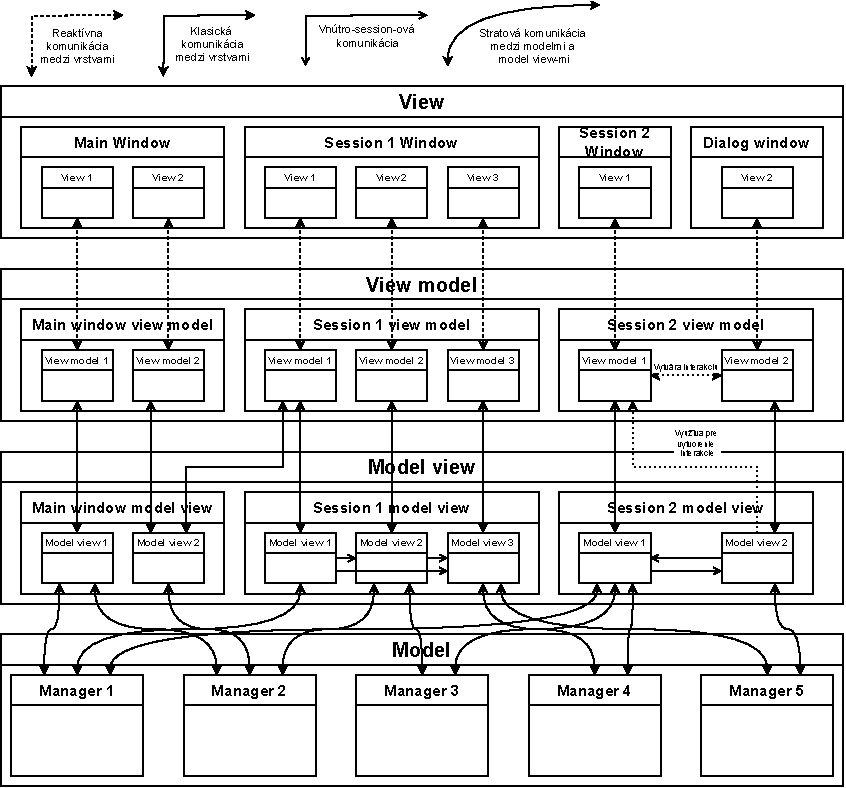
\includegraphics[]{img/priklad_struktury}
\caption{Príklad možnej \uv{mriežkovej} štruktúry aplikácie.} 
\label{obr02:priklad_struktury}
\end{figure}
